\section{Background \& Motivation}
\label{sec:background_motivation}

\subsection{EVM Architecture and Workloads}
\begin{figure}[!htbp]
\centering
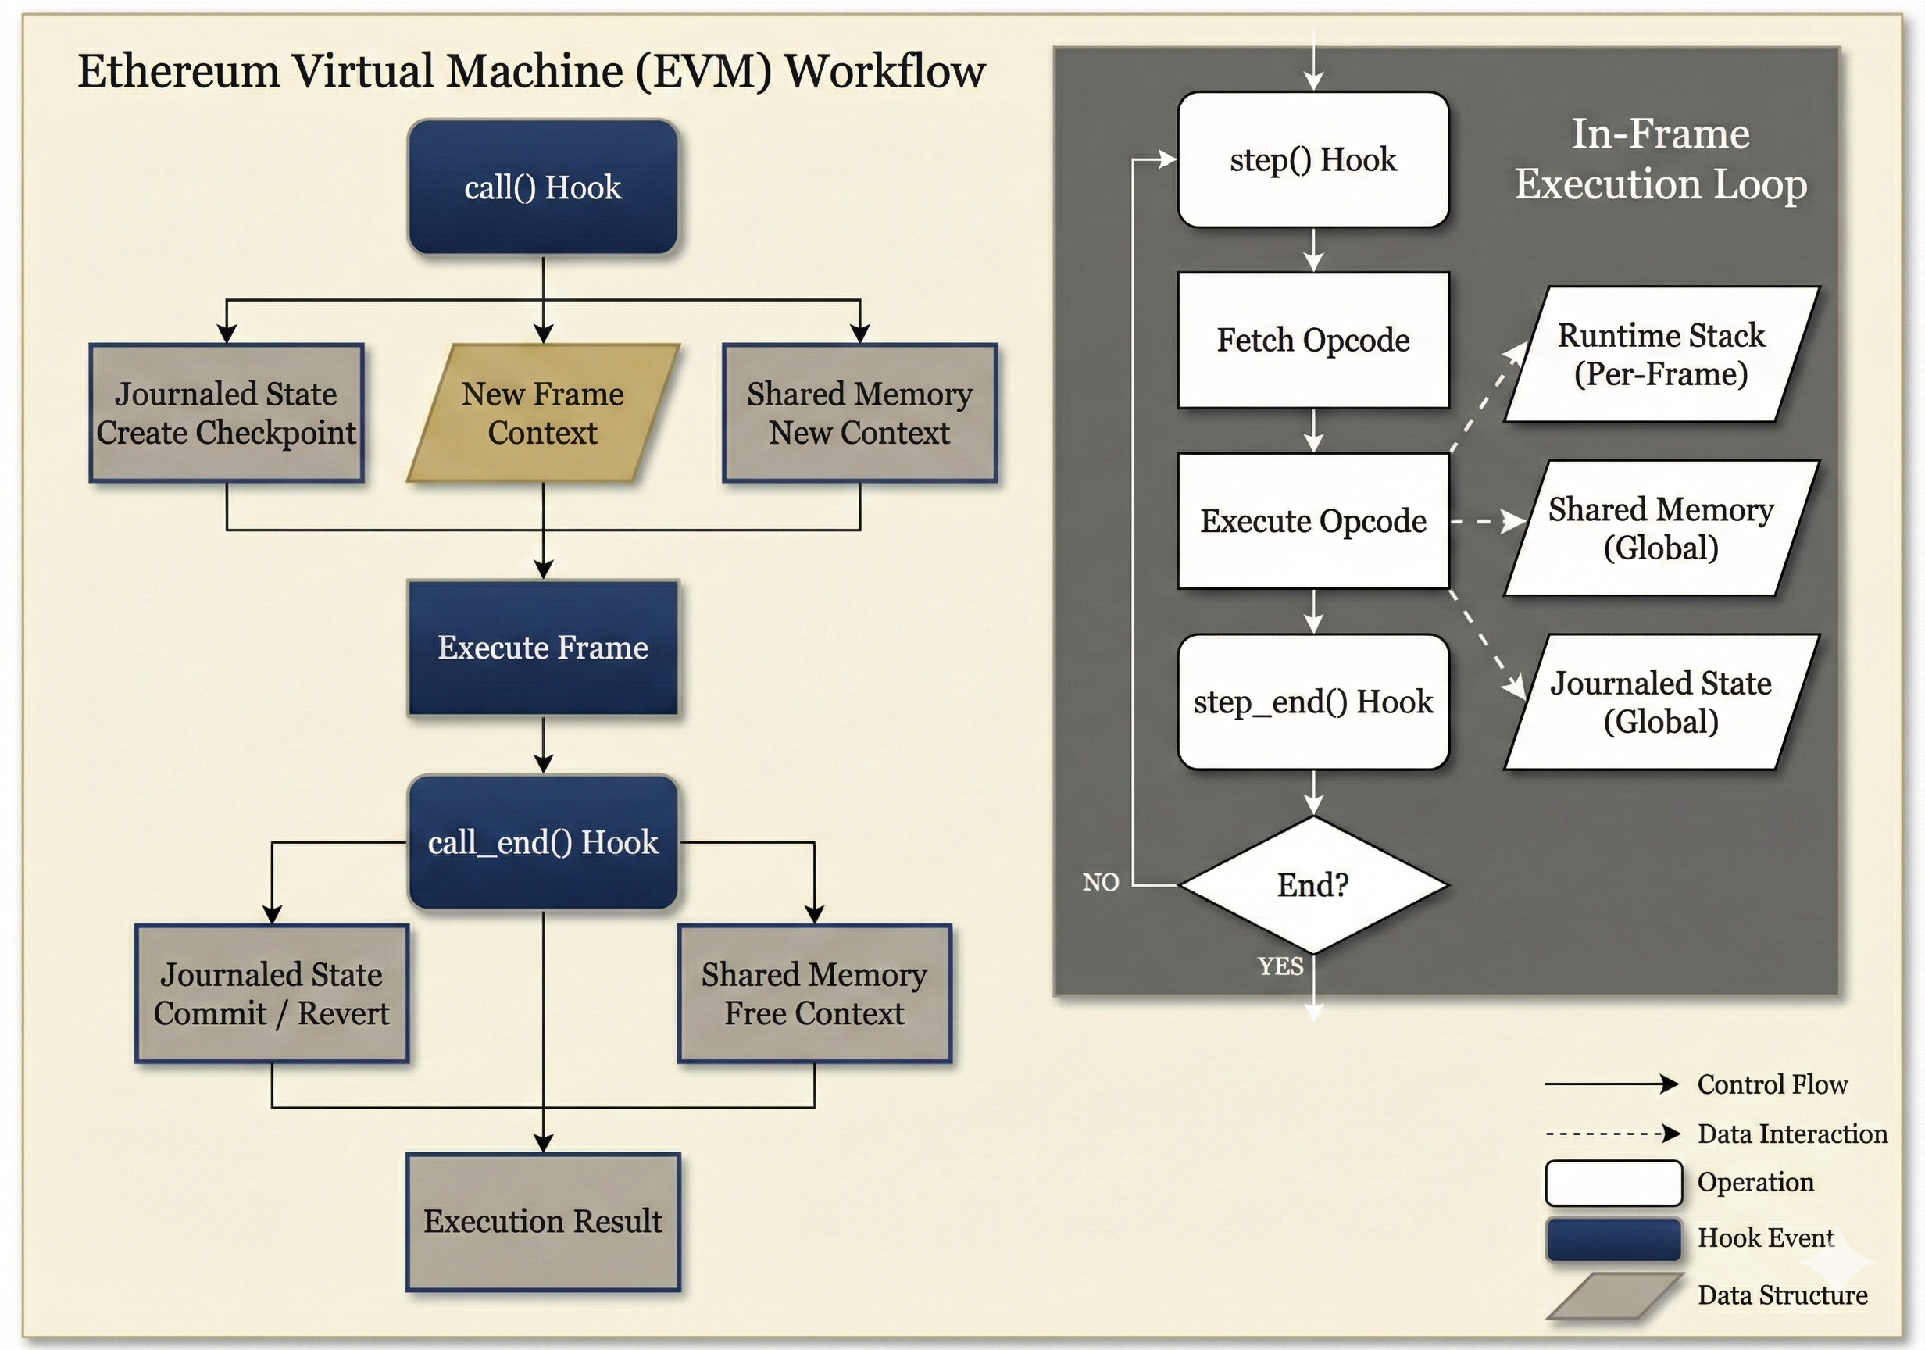
\includegraphics[width=\columnwidth]{raw-figures/EVM.drawio.pdf}
\caption{The EVM execution workflow. The process is partitioned into a high-level frame management lifecycle (left) and a low-level, per-opcode execution loop (right).}
\label{fig:evm-workflow}
\end{figure}


The Ethereum Virtual Machine operates as a quasi-Turing-complete stack machine~\cite{ethereum}. Unlike register-based architectures, the EVM performs all computations on a transient runtime stack using manipulation instructions such as DUP and SWAP to manage operand placement. This design necessitates frequent stack operations that incur significant execution overhead.

Execution is compartmentalized into a hierarchy of call frames. Each frame maintains an isolated memory context and stack while sharing persistent storage access with other frames in the transaction. Resource consumption is metered via gas, which functions as both a validator incentive and a security mechanism against denial-of-service attacks. Gas costs fall into two distinct categories. Static costs are fixed at compile time for computational operations such as arithmetic and stack manipulation. Dynamic costs depend on runtime state, including memory expansion extent and storage access frequency. This distinction is fundamental to our design, as it enables optimization strategies that aggregate static costs while delegating dynamic accounting to native handling logic.

The EVM specification includes a standard hook mechanism to facilitate debugging and tracing. As illustrated in Figure~\ref{fig:evm-workflow}, this interface triggers events at key lifecycle points such as opcode execution and frame transitions. This design enables external components to passively observe execution states and capture data dependencies without requiring invasive modifications to the core interpreter logic.

Given this execution model, the performance characteristics of EVM clients vary depending on their operational role. The Ethereum network depends on node archetypes that exhibit divergent operational characteristics~\cite{eth-nodes-and-clients}. Full nodes operate within fixed block intervals and prioritize the low-latency processing of unpredictable transactions to maintain consensus stability. Archive nodes maintain comprehensive ledger history and emphasize execution throughput to facilitate bulk re-execution of historical states~\cite{geth-sync-modes, eth-archive-node, feng2024slimarchive}.

This operational dichotomy has direct implications for execution acceleration. Full nodes operate in an online mode where execution paths are unknown prior to invocation, precluding ahead-of-time compilation. Acceleration in this context demands minimal response latency while simultaneously generating optimization artifacts for future reuse. Archive nodes operate in a replay mode where execution paths are deterministic and known in advance, enabling aggressive precomputation. Acceleration in this context demands maximum throughput by leveraging cached artifacts across millions of historical transactions. Existing acceleration strategies, however, tend to optimize for one mode at the expense of the other. Systems designed for replay prioritize throughput but lack the responsiveness required for online validation~\cite{feng2024slimarchive}. Conversely, systems targeting online execution prioritize latency but produce ephemeral artifacts with limited reuse potential for historical replay~\cite{forerunner,seer}. A unified acceleration framework must bridge this divide, achieving both low-latency responsiveness and high-throughput batch processing within a single architectural paradigm.

% require \usepackage{booktabs}
\begin{table}[t]
\centering
\caption{Performance degradation of path-driven optimization on modern EVMs. 
Measurements on Uniswap V2 swap (1-hop) demonstrate that artifact overhead 
dominates when baseline execution is fast.}
\label{tab:motivation-overhead}
\small
\resizebox{\columnwidth}{!}{%
\begin{tabular}{llrrr}
\toprule
\textbf{System} & \textbf{Client} & \textbf{Latency} & \textbf{Speedup} & \textbf{Artifact} \\
 & & \textbf{(µs)} & \textbf{(×)} & \textbf{(KB)} \\
\midrule
Native          & Geth         & 398.4   & 1.0×    & --    \\
Forerunner      & Geth         & 68.1    & 5.8×    & 910   \\
\midrule
Native          & Revm         & 62.0    & 1.0×    & --    \\
Forerunner      & Revm         & 39.2    & 1.6×    & 663   \\
\midrule
\textbf{Helios} & \textbf{Revm} & \textbf{31.0} & \textbf{2.0×} & \textbf{70} \\
\bottomrule
\end{tabular}%
}
\end{table}

\subsection{Challenges of EVM Acceleration}

Accelerating EVM execution while preserving semantic correctness presents three interconnected challenges: the \textit{Compilation Limitation}, the \textit{Optimization Dilemma}, and the \textit{Granularity Mismatch}. We examine each in turn.

\subsubsection{The Compilation Limitation}

Contract-level optimization, exemplified by JIT compilation, faces two critical limitations in permissionless blockchain environments. \textbf{First}, JIT compilation can introduce security vulnerabilities. Attackers can construct pathological code patterns, such as deeply nested conditional branches, to trigger exponential compilation complexity. This computational asymmetry allows malicious actors to exhaust validator resources via low-gas transactions, constituting a denial-of-service vector known as JIT bombs~\cite{revmc,monad,evmjit,bnbjit,JITBomb}. \textbf{Second}, JIT compilation risks gas-semantic discrepancies. Aggressive compiler optimizations such as instruction reordering and dead code elimination alter the observable execution trace, violating the strict gas accounting rules that underpin economic consensus. Any systematic deviation from the canonical gas schedule results in incorrect validator compensation and impedes the deployment of production clients~\cite{revmc,monad}.

These constraints suggest that contract-level compilation faces significant challenges in permissionless execution environments. Path-driven optimization offers a potential alternative by restricting acceleration to actually executed paths, thereby bounding optimization costs to the runtime trace and inherently avoiding dead code and unreachable branches. However, path-driven approaches introduce a distinct correctness challenge~\cite{parallelEvm,forerunner,seer}. Cached paths are derived from historical traces, but blockchain state evolves continuously as new transactions modify storage. When runtime conditions diverge from the profiled trace, executing a cached path without verification risks producing incorrect state transitions. This path-divergence problem demands careful mitigation in any path-driven design. Beyond correctness, existing path-driven approaches encounter a second barrier on modern execution engines.

\begin{figure}[b]
\centering
\includegraphics[width=\columnwidth]{raw-figures/pareto_cumulative.pdf}
\caption{Path locality in EVM execution follows an extreme Pareto distribution: the top 1\% of unique paths account for 70\% of frame executions (5,000 mainnet blocks). The shaded region shows deviation from uniform distribution.}
\label{fig:pareto-cumulative}
\end{figure}

\subsubsection{The Optimization Dilemma}
Existing path-driven schemes face a phenomenon we term the \textit{Optimization Dilemma}. On slower engines such as Geth~\cite{geth}, transaction execution dominates end-to-end latency, rendering additional instrumentation costs negligible. A prior path-driven system~\cite{forerunner} achieves a 5.8$\times$ speedup on Geth. However, on highly optimized engines such as Revm~\cite{revm}, execution becomes inexpensive and auxiliary overhead emerges as the primary bottleneck. The same system achieves a more modest 1.6$\times$ on Revm. Table~\ref{tab:motivation-overhead} quantifies this shift using a representative Uniswap V2 swap transaction~\cite{uniswapv2}.

Three categories of auxiliary overhead contribute to this dilemma. \textbf{First}, synchronous tracing dominates the critical path. On Revm, capturing full execution state is approximately six times slower than native execution and nearly ten times slower than optimized execution. Synchronous instrumentation on the critical path tends to negate the speedup from optimization. \textbf{Second}, artifact management incurs substantial fixed costs. Loading and parsing a 663\,KB artifact to accelerate a task completing in tens of microseconds introduces I/O latency that does not scale with execution time. \textbf{Third}, fine-grained concurrency yields limited benefits. We implemented a dependency-graph-driven parallel executor on Revm to evaluate instruction-level parallelism. As shown in Table~\ref{tab:motivation-overhead}, this approach achieves approximately 0.2$\times$ the throughput of sequential execution. The root cause is granularity mismatch. Individual opcode execution requires approximately 20 nanoseconds, while thread synchronization and context switching require hundreds of nanoseconds~\cite{parallelEvm,evmTracer}. Coordination overhead typically exceeds parallel gains at this granularity.

These observations collectively suggest that synchronous tracing, heavyweight artifacts, and fine-grained parallelism present significant challenges for achieving meaningful speedup on high-performance execution engines. Overcoming this dilemma requires fundamentally rethinking where and how optimization occurs relative to the critical execution path.

\subsubsection{The Granularity Mismatch}


Beyond auxiliary overhead, existing path-driven strategies employ transaction-level caching~\cite{forerunner,seer,parallelEvm}, treating the entire execution trace as the atomic optimization unit. This granularity creates a combinatorial challenge where slight variations in call sequences invalidate cached artifacts, often resulting in a use-once-discard lifecycle that limits reuse.

Our analysis of Ethereum mainnet workloads reveals significant redundancy at finer granularity. As shown in Figure~\ref{fig:pareto-cumulative}, frame-level paths follow a Pareto distribution where the top 1\% accounts for over 70\% of execution time. While transaction combinations are vast, individual contract calls function as repetitive building blocks, and shifting the optimization unit to frames amortizes costs across thousands of invocations. However, finer granularity alone does not eliminate cache-flooding risk: adversaries can craft contracts generating numerous unique paths, each triggering insertion without reuse. This attack surface demands robust defenses against adversarial path generation.

\subsection{Our Approach}

The preceding analysis motivates Helios, a path-driven execution engine designed for safety, efficiency, robustness, and versatility. Helios adopts three architectural principles that directly address the challenges above.

To address the \textit{Compilation Limitation}, Helios abandons full JIT compilation in favor of a hybrid execution model. The engine compiles only static-cost instructions into a register-based intermediate representation for acceleration, while delegating dynamic-cost operations to the native interpreter. This separation preserves gas-semantic equivalence by construction. To mitigate the risk of path divergence in a mutable blockchain environment, Helios embeds lightweight \textit{control-flow guards} within optimized paths. These guards verify jump targets against the current execution context and trigger immediate fallback to native execution upon detecting any deviation.

To resolve the \textit{Optimization Dilemma}, Helios decouples instrumentation from the critical path through an asynchronous tracing pipeline that generates optimization artifacts in the background without blocking transaction processing. Leveraging the insight that relevant dependencies are confined to the stack, Helios employs a lightweight tracer that captures necessary data flows without the prohibitive overhead of full memory or storage snapshots. The resulting hot paths are transformed into a register-based intermediate representation that achieves acceleration through direct data access and bulk gas deduction across static instruction sequences.

To overcome the \textit{Granularity Mismatch}, Helios shifts the atomic unit of caching from transactions to call frames. This granularity exploits the high path locality of individual contract calls, converting ephemeral traces into reusable components. To defend against cache-flooding attacks, the system integrates \textit{frequency-based filtering} that admits only statistically significant paths into the acceleration pipeline. This frame-level architecture also unifies the acceleration paradigm, allowing the same guarded artifacts to serve as predictive accelerators for latency-sensitive validators in Online Mode and as deterministic processors for throughput-oriented historical replay in Replay Mode.